\documentclass{zapiski}
\originfo{529}{}{}{2023}
\setcounter{page}{177}
\date{12 îêòÿáðÿ 2023 ã.}

\usepackage[cp1251]{inputenc}
\usepackage[T2A]{fontenc}
\usepackage[russian, english]{babel}

\usepackage{times}
\usepackage{url}
\usepackage{latexsym}
\usepackage{multirow}
\usepackage{lipsum}
\usepackage{graphicx}
\usepackage{amssymb}
\usepackage{hyperref}
\usepackage{multirow}
\usepackage{booktabs}
\usepackage{tabularx}
\usepackage{caption}
\usepackage{cite}

\usepackage{paralist}
\usepackage{subcaption}
\usepackage{xcolor,colortbl}
\usepackage{array}
%\usepackage{captionof}
%\usepackage{multirow}
\usepackage{setspace}

\usepackage{placeins}

\usepackage{tikz}
\usepackage{pgfplots}

\usepackage{array}
\newcolumntype{H}{>{\setbox0=\hbox\bgroup}c<{\egroup}@{}}
\newcolumntype{Z}{>{\setbox0=\hbox\bgroup}c<{\egroup}@{\hspace*{-\tabcolsep}}}

\renewcommand{\UrlFont}{\ttfamily\small}
\newcommand{\cm}[1]{\textcolor{red}{#1}}
\newcommand{\bm}[1]{\textcolor{blue}{#1}}
\newcommand{\naacl}[1]{#1}

\usepackage{float}
\restylefloat{table}

\english

\begin{document}

\title[Your Paper Short Title]{Your Paper Full Title}


\author[Author]{Full Name}
\address[F.~Name]{Address}
\email{email}

\begin{abstract}
Abstract of your paper.
\end{abstract}

\keywords{key  \and words.}

\maketitle

\section{Introduction}\label{sec:intro}

Below you could find a few samples of citations.

Hussain et al. \cite{hussain2017automatic} present a crowdsourced dataset of such advertisements, including images and videos, and formulate several annotation tasks: topic detection, sentiment type detection, symbolism recognition, strategy analysis, slogan annotation, and Q/A for texts related to the ads' messages and motivation. We focus on the first three tasks, each of which can be formulated as a classification problem.
A preliminary version of this work has appeared in \cite{savchenko2020ad}. 

Fig.~\ref{fig:model} is a sample for image inclusion. Tab.~\ref{tab:ocr} is a sample of table inclusion. Fig.~\ref{tab:topics_sentiments_overall_accuracy} is a sample of tikz figure inclusion.

\begin{figure}[!tbh]
    \centering
    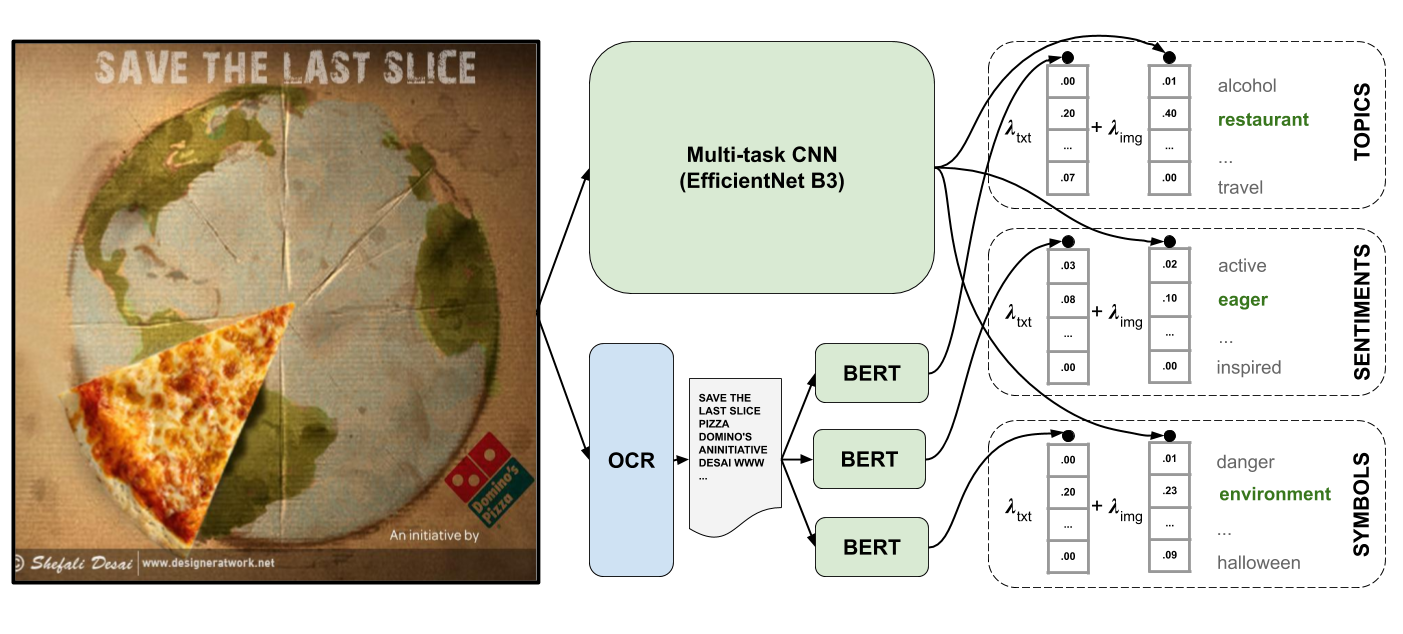
\includegraphics[width=0.95\textwidth]{pic/model.png}\vspace{-.5cm}

    \caption{The proposed blending scheme.}
    \label{fig:model}\vspace{-.3cm}
\end{figure}



\begin{table}[!tbh]\setlength{\tabcolsep}{2pt}
\begin{tabular}{p{.17\linewidth}|p{.79\linewidth}}
\hline
\emph{Tesseract}\newline  \cite{smith2007overview} & 
Maybe all that raven
wants is to wet its
beak in a’cold glass of milk.
poe mea lo EISsTo) aU eg
\\\hline
EAST+\newline\emph{Tesseract}\newline\cite{kopeykina2019automatic} & 
Maybe are Gein) eu SH Hostel S to wet its ake cold Me TS 10a milk. eee me glass 0) aa Penal see 
\\\hline
PSENet \newline \cite{wang2019shape} &  Elle that eV WM eMey iy is 10 Wed Mey in beak | Ey milk. of (eek glass | ranlll@a a me al eee) glass be at jeffreycombs-com  \\ \hline
EasyOCR \newline \cite{easyocr} &  Maybe all that raven poe me a glass ofmik? beak in a cold glass ofmik. wants is to wet its seen 3t jefieycomlzesolm  \\ \hline
Charnet \newline \cite{xing2019convolutional} & MAYBE ALL THAT RAVEN WANTS WET ITS BEAKIN COLD GLASS MILK POE GLASS MILK? SEEN ATJ COM 
\\ \hline
CloudVision \newline \cite{otani2018} & Maybe all that raven
wants is to wet its
beak in a cold glass of milk.
poe me a glass of milk?
seen at jeffreycombs.com
 \\\hline
\end{tabular}

\caption{Sample  texts obtained via OCR/captioning.}\label{tab:ocr}
\end{table}





\begin{figure}[!tbh] 
\centering
    % \includegraphics[width=0.5\textwidth]{pic/Fig_ads_221_f1.eps}
    \tikzset{dashdot/.style={dash pattern=on .4pt off 3pt on 4pt off 3pt}}
\pgfplotsset{every tick label/.append style={font=\footnotesize}}
\pgfplotsset{every axis legend/.append style={font=\footnotesize,draw=none}}
\pgfplotsset{every axis label/.append style={font=\footnotesize}}

\pgfplotsset{every axis/.append style={width=\linewidth, height={.6\linewidth}, grid=major, grid style={dashed,gray!25}, legend cell align=left, legend columns=1}}
\pgfplotsset{every axis x label/.append style={at={(axis description cs:1.0,0.1)}, anchor=north east}}
\pgfplotsset{every axis y label/.append style={at={(axis description cs:-0.,0.5)}, anchor=north}}

\begin{tikzpicture}
  \begin{axis}[
    height=4cm,
      xlabel={Threshold $t_0$},
      ylabel={F1-score},
      enlargelimits=false,
      % ymin=1,
      ytick={0,0.05,0.1,0.15},yticklabels={0,0.05,0.1,0.15},
      % ytick={1,50,100},yticklabels={1,50,100},
      xmax=1.0,xmin=0,
      % x tick label style={rotate=90,anchor=east} % Display labels sideways
    ]
    \addplot[color=blue,line width=0.9pt,mark size=1.5pt,mark=star] table[x index=0,y index=1] {pic/symbols_fscore_on_threshold.csv};
    \addplot[color=red,line width=0.9pt,mark size=1pt,mark=*] table[x index=0,y index=2] {pic/symbols_fscore_on_threshold.csv};
    \addplot[color=green!60!black,line width=0.9pt,mark size=1pt,mark=triangle] table[x index=0,y index=3] {pic/symbols_fscore_on_threshold.csv};
    \legend{{MobileNet v1},{Inception v3},{EfficientNet-B3}};
  \end{axis}
\end{tikzpicture}   
    
	\caption{F1-score for image-based symbol recognition (221 categories).} 
	\label{visual-221-f1}
% \end{figure}

% \begin{table}[!t]
    \footnotesize\setlength{\tabcolsep}{2.8pt}
    \begin{tabular}{|c|c|c|}
    \hline
        CNN & Topics & Sentiments \\
        \hline
        Baseline~\cite{hussain2017automatic} & 60.34& 27.92\\
        Curriculum learning~\cite{10.1007/978-3-030-01216-8_36} & --- & 27.96\\
        \hline
        ResNet-50 & 53.90 & 34.34 \\
        Resnet-152 & 52.67 & 27.58 \\
        Resnet-152 V2 & 52.12 & 27.64 \\
        MobileNet v1& 50.56 & 33.50\\
        MobileNet v2 & 54.76  & \textbf{34.58}\\
        EfficientNet-B0 & 60.06 & 34.03\\
        EfficientNet-B3 & \textbf{62.62} & 34.12 \\
        \hline
        Our multitask model & \textbf{62.99} & \textbf{36.27} \\ \hline
    \end{tabular}
    \captionof{table}{Image-based topic/sentiment classification.}
    \label{tab:topics_sentiments_overall_accuracy}
\end{figure}



\section*{Acknowledgments}
The work has been supported by the Fund grant \#XXX. 

% \bibliographystyle{amsplain}
% \bibliography{anthology,eacl2021}

\providecommand{\bysame}{\leavevmode\hbox to3em{\hrulefill}\thinspace}
\providecommand{\MR}{\relax\ifhmode\unskip\space\fi MR }
% \MRhref is called by the amsart/book/proc definition of \MR.
\providecommand{\MRhref}[2]{%
  \href{http://www.ams.org/mathscinet-getitem?mr=#1}{#2}
}
\providecommand{\href}[2]{#2}
\begin{thebibliography}{10}

\bibitem{ahuja2018understanding}
Karuna Ahuja, Karan Sikka, Anirban Roy, and Ajay Divakaran, \emph{Understanding
  visual ads by aligning symbols and objects using co-attention}, arXiv
  preprint arXiv:1807.01448 (2018).

\bibitem{antol2015vqa}
Stanislaw Antol, Aishwarya Agrawal, Jiasen Lu, Margaret Mitchell, Dhruv Batra,
  C~Lawrence Zitnick, and Devi Parikh, \emph{{VQA}: Visual question answering},
  Proceedings of the IEEE International Conference on Computer Vision (ICCV),
  2015, pp.~2425--2433.

\bibitem{baltruvsaitis2018multimodal}
Tadas Baltru{\v{s}}aitis, Chaitanya Ahuja, and Louis-Philippe Morency,
  \emph{Multimodal machine learning: A survey and taxonomy}, IEEE Transactions
  on Pattern Analysis and Machine Intelligence \textbf{41} (2018), no.~2,
  423--443.

\bibitem{fastTextEmbeddings}
Piotr Bojanowski, Edouard Grave, Armand Joulin, and Tomas Mikolov,
  \emph{Enriching word vectors with subword information}, Transactions of the
  Association for Computational Linguistics \textbf{5} (2017), 135--146.

\bibitem{saussure1916course}
Ferdinand de~Saussure, \emph{Course in general linguistics}, Duckworth, London,
  1983, (trans. Roy Harris).

\bibitem{demochkina2021mobileemotiface}
Polina Demochkina and Andrey~V Savchenko, \emph{{MobileEmotiFace}: Efficient
  facial image representations in video-based emotion recognition on mobile
  devices}, Proceedings of Pattern Recognition. ICPR International Workshops
  and Challenges: Virtual Event, January 10--15, 2021, Proceedings, Part V,
  Springer, 2021, pp.~266--274.

\bibitem{devlin2018bert}
Jacob Devlin, Ming-Wei Chang, Kenton Lee, and Kristina Toutanova, \emph{Bert:
  Pre-training of deep bidirectional transformers for language understanding},
  2018.

\bibitem{dey2018don}
Arka~Ujjal Dey, Suman~K Ghosh, and Ernest Valveny, \emph{Don't only feel read:
  Using scene text to understand advertisements}, arXiv preprint
  arXiv:1806.08279 (2018).

\bibitem{dey2019visual}
Arka~Ujjal Dey, Suman~Kumar Ghosh, Ernest Valveny, and Gaurav Harit,
  \emph{Beyond visual semantics: Exploring the role of scene text in image
  understanding}, 2019.

\bibitem{he2016deep}
Kaiming He, Xiangyu Zhang, Shaoqing Ren, and Jian Sun, \emph{Deep residual
  learning for image recognition}, Proceedings of the IEEE Conference on
  Computer Vision and Pattern Recognition (CVPR), 2016, pp.~770--778.

\bibitem{howard2017mobilenets}
Andrew~G Howard, Menglong Zhu, Bo~Chen, Dmitry Kalenichenko, Weijun Wang,
  Tobias Weyand, Marco Andreetto, and Hartwig Adam, \emph{Mobilenets: Efficient
  convolutional neural networks for mobile vision applications}, arXiv preprint
  arXiv:1704.04861 (2017).

\bibitem{hussain2017automatic}
Zaeem Hussain, Mingda Zhang, Xiaozhong Zhang, Keren Ye, Christopher Thomas,
  Zuha Agha, Nathan Ong, and Adriana Kovashka, \emph{Automatic understanding of
  image and video advertisements}, Proceedings of the IEEE Conference on
  Computer Vision and Pattern Recognition (CVPR), 2017, pp.~1705--1715.

\bibitem{ivanov2015extracting}
VV~Ivanov, EV~Tutubalina, NR~Mingazov, and IS~Alimova, \emph{Extracting
  aspects, sentiment and categories of aspects in user reviews about
  restaurants and cars}, Komp'juternaja Lingvistika i Intellektual'nye
  Tehnologii, 2015, pp.~22--33.

\bibitem{jabeen2023review}
Summaira Jabeen, Xi~Li, Muhammad~Shoib Amin, Omar Bourahla, Songyuan Li, and
  Abdul Jabbar, \emph{A review on methods and applications in multimodal deep
  learning}, ACM Transactions on Multimedia Computing, Communications and
  Applications \textbf{19} (2023), no.~2s, 1--41.

\bibitem{easyocr}
JaidedAI, \emph{{EasyOCR}: Ready-to-use ocr with 70+ languages supported
  including chinese, japanese, korean and thai.},
  \url{https://github.com/JaidedAI/EasyOCR}, 2020.

\bibitem{kalra2020understanding}
Kanika Kalra, Bhargav Kurma, Silpa~Vadakkeeveetil Sreelatha, Manasi Patwardhan,
  and Shirish Karande, \emph{Understanding advertisements with {BERT}},
  Proceedings of the 58th Annual Meeting of the Association for Computational
  Linguistics, 2020, pp.~7542--7547.

\bibitem{karpov2022exploring}
Aleksei Karpov and Ilya Makarov, \emph{Exploring efficiency of vision
  transformers for self-supervised monocular depth estimation}, Proceedings of
  International Symposium on Mixed and Augmented Reality (ISMAR), IEEE, 2022,
  pp.~711--719.

\bibitem{savchenko2014neural}
Ya~I Khokhlova and AV~Savchenko, \emph{About neural-network algorithms
  application in viseme classification problem with face video in audiovisual
  speech recognition systems}, Optical Memory and Neural Networks \textbf{23}
  (2014), 34--42.

\bibitem{kiela2019supervised}
Douwe Kiela, Suvrat Bhooshan, Hamed Firooz, and Davide Testuggine,
  \emph{Supervised multimodal bitransformers for classifying images and text},
  arXiv preprint arXiv:1909.02950 (2019).

\bibitem{kingma2014adam}
Diederik~P Kingma and Jimmy Ba, \emph{Adam: A method for stochastic
  optimization}, International Conference on Learning Representations (ICLR),
  2015.

\bibitem{kopeykina2019automatic}
Lyudmila Kopeykina and Andrey~V Savchenko, \emph{Automatic privacy detection in
  scanned document images based on deep neural networks}, Proceedings of the
  International Russian Automation Conference (RusAutoCon), IEEE, 2019,
  pp.~1--6.

\bibitem{li2019visualbert}
Liunian~Harold Li, Mark Yatskar, Da~Yin, Cho-Jui Hsieh, and Kai-Wei Chang,
  \emph{Visual{BERT}: A simple and performant baseline for vision and
  language}, arXiv preprint arXiv:1908.03557 (2019).

\bibitem{liang2019learning}
Paul~Pu Liang, Zhun Liu, Yao-Hung~Hubert Tsai, Qibin Zhao, Ruslan
  Salakhutdinov, and Louis-Philippe Morency, \emph{Learning representations
  from imperfect time series data via tensor rank regularization}, Proceedings
  of the 57th Annual Meeting of the Association for Computational Linguistics,
  2019, pp.~1569--1576.

\bibitem{liang2018multimodal}
Paul~Pu Liang, Ziyin Liu, AmirAli~Bagher Zadeh, and Louis-Philippe Morency,
  \emph{Multimodal language analysis with recurrent multistage fusion},
  Proceedings of the 2018 Conference on Empirical Methods in Natural Language
  Processing, 2018, pp.~150--161.

\bibitem{liu2023survey}
Yang Liu, Yao Zhang, Yixin Wang, Feng Hou, Jin Yuan, Jiang Tian, Yang Zhang,
  Zhongchao Shi, Jianping Fan, and Zhiqiang He, \emph{A survey of visual
  transformers}, IEEE Transactions on Neural Networks and Learning Systems
  (2023).

\bibitem{liu2019roberta}
Yinhan Liu, Myle Ott, Naman Goyal, Jingfei Du, Mandar Joshi, Danqi Chen, Omer
  Levy, Mike Lewis, Luke Zettlemoyer, and Veselin Stoyanov, \emph{{RoBERTa}: A
  robustly optimized {BERT} pretraining approach}, 2019.

\bibitem{mcduff2014predicting}
Daniel McDuff, Rana El~Kaliouby, Jeffrey~F Cohn, and Rosalind~W Picard,
  \emph{Predicting ad liking and purchase intent: Large-scale analysis of
  facial responses to ads}, IEEE Transactions on Affective Computing \textbf{6}
  (2014), no.~3, 223--235.

\bibitem{mikolov2013efficient}
Tomas Mikolov, Kai Chen, Greg Corrado, and Jeffrey Dean, \emph{Efficient
  estimation of word representations in vector space}, arXiv preprint
  arXiv:1301.3781 (2013).

\bibitem{mikolov2013distributed}
Tomas Mikolov, Ilya Sutskever, Kai Chen, Greg~S Corrado, and Jeff Dean,
  \emph{Distributed representations of words and phrases and their
  compositionality}, Advances in neural information processing systems, 2013,
  pp.~3111--3119.

\bibitem{mishra2020learning}
Shaunak Mishra, Manisha Verma, Yichao Zhou, Kapil Thadani, and Wei Wang,
  \emph{Learning to create better ads: Generation and ranking approaches for ad
  creative refinement},  (2020), 2653--2660.

\bibitem{olson2008visual}
Lester~C Olson, Cara~A Finnegan, and Diane~S Hope, \emph{Visual rhetoric: A
  reader in communication and american culture}, Sage, 2008.

\bibitem{gpt4}
OpenAI, \emph{{GPT-4} technical report}, arXiv preprint arXiv:2303.08774
  (2023).

\bibitem{otani2018}
Mayu Otani, Yuki Iwazaki, and Kota Yamaguchi, \emph{Unreasonable effectiveness
  of {OCR} in visual advertisement understanding}, 2018.

\bibitem{10.1007/978-3-030-01216-8_36}
Rameswar Panda, Jianming Zhang, Haoxiang Li, Joon-Young Lee, Xin Lu, and
  Amit~K. Roy-Chowdhury, \emph{Contemplating visual emotions: Understanding and
  overcoming dataset bias}, Proceedings of European Conference on Computer
  Vision (ECCV) (Cham) (Vittorio Ferrari, Martial Hebert, Cristian
  Sminchisescu, and Yair Weiss, eds.), Springer International Publishing, 2018,
  pp.~594--612.

\bibitem{scikit-learn}
F.~Pedregosa, G.~Varoquaux, A.~Gramfort, V.~Michel, B.~Thirion, O.~Grisel,
  M.~Blondel, P.~Prettenhofer, R.~Weiss, V.~Dubourg, J.~Vanderplas, A.~Passos,
  D.~Cournapeau, M.~Brucher, M.~Perrot, and E.~Duchesnay, \emph{Scikit-learn:
  Machine learning in {P}ython}, Journal of Machine Learning Research
  \textbf{12} (2011), 2825--2830.

\bibitem{plummer2015flickr30k}
Bryan~A Plummer, Liwei Wang, Chris~M Cervantes, Juan~C Caicedo, Julia
  Hockenmaier, and Svetlana Lazebnik, \emph{Flickr30k entities: Collecting
  region-to-phrase correspondences for richer image-to-sentence models},
  Proceedings of the IEEE international conference on computer vision, 2015,
  pp.~2641--2649.

\bibitem{poels2006capture}
Karolien Poels and Siegfried Dewitte, \emph{How to capture the heart? reviewing
  20 years of emotion measurement in advertising}, Journal of Advertising
  Research \textbf{46} (2006), no.~1, 18--37.

\bibitem{radford2021learning}
Alec Radford, Jong~Wook Kim, Chris Hallacy, Aditya Ramesh, Gabriel Goh,
  Sandhini Agarwal, Girish Sastry, Amanda Askell, Pamela Mishkin, Jack Clark,
  et~al., \emph{Learning transferable visual models from natural language
  supervision}, Proceedings of International Conference on Machine Learning
  (ICML), PMLR, 2021, pp.~8748--8763.

\bibitem{radford2023robust}
Alec Radford, Jong~Wook Kim, Tao Xu, Greg Brockman, Christine McLeavey, and
  Ilya Sutskever, \emph{Robust speech recognition via large-scale weak
  supervision}, Proceedings of International Conference on Machine Learning
  (ICML), PMLR, 2023, pp.~28492--28518.

\bibitem{Rajapakse2020}
Thilina Rajapakse, \emph{Simple transformers}, 2020.

\bibitem{rusnachenko-etal-2019-distant}
Nicolay Rusnachenko, Natalia Loukachevitch, and Elena Tutubalina, \emph{Distant
  supervision for sentiment attitude extraction}, Proceedings of the
  International Conference on Recent Advances in Natural Language Processing
  (RANLP 2019) (Varna, Bulgaria) (Ruslan Mitkov and Galia Angelova, eds.),
  INCOMA Ltd., September 2019, pp.~1022--1030.

\bibitem{sakhovskiy2021kfu}
Andrey Sakhovskiy, Zulfat Miftahutdinov, and Elena Tutubalina, \emph{Kfu nlp
  team at smm4h 2021 tasks: Cross-lingual and cross-modal bert-based models for
  adverse drug effects}, Proceedings of the Sixth Social Media Mining for
  Health (\# SMM4H) Workshop and Shared Task, 2021, pp.~39--43.

\bibitem{sakhovskiy2022multimodal}
Andrey Sakhovskiy and Elena Tutubalina, \emph{Multimodal model with text and
  drug embeddings for adverse drug reaction classification}, Journal of
  Biomedical Informatics \textbf{135} (2022), 104182.

\bibitem{sandler2018mobilenetv2}
Mark Sandler, Andrew Howard, Menglong Zhu, Andrey Zhmoginov, and Liang-Chieh
  Chen, \emph{Mobilenetv2: Inverted residuals and linear bottlenecks},
  Proceedings of the IEEE conference on Computer Vision and Pattern Recognition
  (CVPR), 2018, pp.~4510--4520.

\bibitem{savchenko2023facial}
Andrey Savchenko, \emph{Facial expression recognition with adaptive frame rate
  based on multiple testing correction}, International Conference on Machine
  Learning, PMLR, 2023, pp.~30119--30129.

\bibitem{savchenko2020ad}
Andrey Savchenko, Anton Alekseev, Sejeong Kwon, Elena Tutubalina, Evgeny
  Myasnikov, and Sergey Nikolenko, \emph{Ad lingua: Text classification
  improves symbolism prediction in image advertisements}, Proceedings of the
  28th International Conference on Computational Linguistics, 2020,
  pp.~1886--1892.

\bibitem{savchenko2022mt}
Andrey~V Savchenko, \emph{{MT-EmotiEffNet} for multi-task human affective
  behavior analysis and learning from synthetic data}, Proceedings of European
  Conference on Computer Vision Workshops (ECCVW), Springer, 2022, pp.~45--59.

\bibitem{savchenko2022preference}
Andrey~V Savchenko, Kirill~V Demochkin, and Ivan~S Grechikhin, \emph{Preference
  prediction based on a photo gallery analysis with scene recognition and
  object detection}, Pattern Recognition \textbf{121} (2022), 108248.

\bibitem{savchenko2019criterion}
Vladimir~V Savchenko and Andrey~V Savchenko, \emph{Criterion of significance
  level for selection of order of spectral estimation of entropy maximum},
  Radioelectronics and Communications Systems \textbf{62} (2019), no.~5,
  223--231.

\bibitem{singh2020mmf}
Amanpreet Singh, Vedanuj Goswami, Vivek Natarajan, Yu~Jiang, Xinlei Chen, Meet
  Shah, Marcus Rohrbach, Dhruv Batra, and Devi Parikh, \emph{{MMF}: A
  multimodal framework for vision and language research},
  \url{https://github.com/facebookresearch/mmf}, 2020.

\bibitem{smith2007overview}
Ray Smith, \emph{An overview of the {Tesseract} {OCR} engine}, Proceedings of
  the International Conference on Document Analysis and Recognition (ICDAR),
  vol.~2, IEEE, 2007, pp.~629--633.

\bibitem{suhr2019corpus}
Alane Suhr, Stephanie Zhou, Ally Zhang, Iris Zhang, Huajun Bai, and Yoav Artzi,
  \emph{A corpus for reasoning about natural language grounded in photographs},
  Proceedings of the 57th Annual Meeting of the Association for Computational
  Linguistics, 2019, pp.~6418--6428.

\bibitem{tan2019efficientnet}
Mingxing Tan and Quoc~V Le, \emph{{EfficientNet}: Rethinking model scaling for
  convolutional neural networks},  (2019), 6105--6114.

\bibitem{tsai2018learning}
Yao-Hung~Hubert Tsai, Paul~Pu Liang, Amir Zadeh, Louis-Philippe Morency, and
  Ruslan Salakhutdinov, \emph{Learning factorized multimodal representations},
  International Conference on Learning Representations (ICLR), 2018.

\bibitem{tutubalina2015inferring}
Elena Tutubalina and Sergey Nikolenko, \emph{Inferring sentiment-based priors
  in topic models}, Mexican International Conference on Artificial
  Intelligence, Springer, 2015, pp.~92--104.

\bibitem{wang2019shape}
Wenhai Wang, Enze Xie, Xiang Li, Wenbo Hou, Tong Lu, Gang Yu, and Shuai Shao,
  \emph{Shape robust text detection with progressive scale expansion network},
  2019.

\bibitem{williamson1978}
Judith Williamson, \emph{Decoding advertisement}, 1978.

\bibitem{Wolf2019HuggingFacesTS}
Thomas Wolf, Lysandre Debut, Victor Sanh, Julien Chaumond, Clement Delangue,
  Anthony Moi, Pierric Cistac, Tim Rault, R'emi Louf, Morgan Funtowicz, and
  Jamie Brew, \emph{Huggingface's transformers: State-of-the-art natural
  language processing}, ArXiv \textbf{abs/1910.03771} (2019).

\bibitem{xiao2023exploring}
Lin Xiao, Xiaofeng Li, and Yucheng Zhang, \emph{Exploring the factors
  influencing consumer engagement behavior regarding short-form video
  advertising: A big data perspective}, Journal of Retailing and Consumer
  Services \textbf{70} (2023), 103170.

\bibitem{xing2019convolutional}
Linjie Xing, Zhi Tian, Weilin Huang, and Matthew~R Scott, \emph{Convolutional
  character networks}, Proceedings of the IEEE International Conference on
  Computer Vision (ICCV), 2019, pp.~9126--9136.

\bibitem{yang2023emoset}
Jingyuan Yang, Qirui Huang, Tingting Ding, Dani Lischinski, Danny Cohen-Or, and
  Hui Huang, \emph{{EmoSet}: A large-scale visual emotion dataset with rich
  attributes}, Proceedings of the IEEE/CVF International Conference on Computer
  Vision (ICCV), 2023, pp.~20383--20394.

\bibitem{8869939}
K.~{Ye}, N.~{Honarvar Nazari}, J.~{Hahn}, Z.~{Hussain}, M.~{Zhang}, and
  A.~{Kovashka}, \emph{Interpreting the rhetoric of visual advertisements},
  IEEE Transactions on Pattern Analysis and Machine Intelligence (2019), 1--1.

\bibitem{ye2018story}
Keren Ye, Kyle Buettner, and Adriana Kovashka, \emph{Story understanding in
  video advertisements}, arXiv preprint arXiv:1807.11122 (2018).

\bibitem{ye2018advise}
Keren Ye and Adriana Kovashka, \emph{Advise: Symbolism and external knowledge
  for decoding advertisements}, Proceedings of the European Conference on
  Computer Vision (ECCV), 2018, pp.~837--855.

\bibitem{zadeh2018multimodal}
AmirAli~Bagher Zadeh, Paul~Pu Liang, Soujanya Poria, Erik Cambria, and
  Louis-Philippe Morency, \emph{Multimodal language analysis in the wild:
  Cmu-mosei dataset and interpretable dynamic fusion graph}, Proceedings of the
  56th Annual Meeting of the Association for Computational Linguistics (Volume
  1: Long Papers), 2018, pp.~2236--2246.

\bibitem{zellers2019recognition}
Rowan Zellers, Yonatan Bisk, Ali Farhadi, and Yejin Choi, \emph{From
  recognition to cognition: Visual commonsense reasoning}, Proceedings of the
  IEEE Conference on Computer Vision and Pattern Recognition (CVPR), 2019,
  pp.~6720--6731.

\bibitem{zhang2018equal}
Mingda Zhang, Rebecca Hwa, and Adriana Kovashka, \emph{Equal but not the same:
  Understanding the implicit relationship between persuasive images and text},
  arXiv preprint arXiv:1807.08205 (2018).

\bibitem{zhou2017east}
Xinyu Zhou, Cong Yao, He~Wen, Yuzhi Wang, Shuchang Zhou, Weiran He, and Jiajun
  Liang, \emph{{EAST}: an efficient and accurate scene text detector},
  Proceedings of the IEEE Conference on Computer Vision and Pattern Recognition
  (CVPR), 2017, pp.~5551--5560.

\bibitem{zhou2020recommending}
Yichao Zhou, Shaunak Mishra, Manisha Verma, Narayan Bhamidipati, and Wei Wang,
  \emph{Recommending themes for ad creative design via visual-linguistic
  representations}, Proceedings of The Web Conference (WWW), 2020,
  pp.~2521--2527.

\end{thebibliography}

\end{document}

À. Àëåêñååâ, À. Ñàâ÷åíêî, Å. Òóòóáàëèíà, Å. Ìÿñíèêîâ, Ñ. Íèêîëåíêî. Îáúåäèíåíèå ïðåäñêàçàíèé óëó÷øàåò ïîíèìàíèå ìóëüòèìîäàëüíîãî ðåêëàìíîãî êîíòåíòà

\begin{abstract}
Ðåêëàìíàÿ èíäóñòðèÿ èñïîëüçóåò íåñêîëüêî ìîäàëüíîñòåé êîíòåíòà äëÿ äîñòàâêè ïîäðàçóìåâàåìûõ ñîîáùåíèé: èçîáðàæåíèÿ, âèäåî, òåêñò, ìóçûêà, è âñå ýòî âìåñòå âçÿòîå. ``Äåêîäèðîâàíèå'' ñîîáùåíèÿ, ïîäðàçóìåâàåìîãî â ìóëüòèìîäàëüíîì êîíòåíòå, ÷àñòî òðåáóåò àíàëèçà êàê òåêñòîâûõ, òàê è âèçóàëüíûõ åãî êîìïîíåíòîâ. Ìû èçó÷àåì çàäà÷è ðàñïîçíàâàíèÿ ìóëüòèìîäàëüíîãî ñèìâîëèçìà, îáíàðóæåíèÿ òåì è êëàññèôèêàöèè òîíàëüíîñòè. Ðóêîâîäñòâóÿñü ðàçíèöåé â ÷àñòÿõ ñîîáùåíèÿ, ïåðåäàâàåìûõ ðàçíûìè ìîäàëüíîñòÿìè â ðåêëàìíûõ îáúÿâëåíèÿõ, ìû îáó÷àåì îòäåëüíûå ìîäåëè äëÿ èçîáðàæåíèé è òåêñòîâ è çíà÷èòåëüíî óëó÷øàåì ðåçóëüòàòû, ñìåøèâàÿ ïðîãíîçû íà îñíîâå èçîáðàæåíèé è òåêñòà (ñ àâòîìàòè÷åñêè ðàñïîçíàííûì òåêñòîì), ÷òî äàåò ýêñïåðèìåíòàëüíîå ïîäòâåðæäåíèå íàøåãî ïîäõîäà.
\end{abstract}

\keywords{ìóëüòèìîäàëüíîå ìàøèííîå îáó÷åíèå \and ïîíèìàíèå ðåêëàìíîãî êîíòåíòà \and ðàñïîçíàâàíèå òåìàòèêè \and òîíàëüíîñòü òåêñòà \and êëàññèôèêàöèÿ òîíàëüíîñòè}